\subsection{Query complexity}
\label{sec:query-complexity}

In this section and the next, we prove the following first result.
\begin{contribution}[label=thm:cube,restate=TheoremKSUMCube]
There exist linear decision trees of depth \(O(n^3\log^2 n)\) solving
the \(k\)-SUM and the \(k\)-LDT problems. Furthermore, for the \(k\)-SUM
problem there
exists an $\tilde{O}(n^{\ceil{\frac{k}{2}}+8})$ Las Vegas algorithm in
the word-RAM model expected to perform $O(n^3 \log^2 n)$ linear queries on the input.
This algorithm also solves the \(k\)-LDT problem within the same time bounds
provided the coefficients of the underlying linear equation are constant rational numbers.
\end{contribution}


\subsubsection{Algorithm outline}
For a fixed set of hyperplanes \(\Hy\) and given input vertex \(q\) in \(\R^n\),
Meiser's algorithm allows us to determine the cell of the arrangement
$\arrangement(\Hy)$ that contains $q$ in its interior (or that \emph{is} $q$ if
$q$ is a $0$-cell of $\arrangement(\Hy)$), that is, the positions $\sigma(H,q) \in
\signset$ of \(q\) with respect to all hyperplanes $H \in \Hy$. In the \(k\)-SUM
problem, the set $\Hy$ is the set of $\Theta(n^k)$ hyperplanes with equations of the
form $x_{i_1} + x_{i_2} + \cdots + x_{i_k} = 0$.
These equations can be modified accordingly for \(k\)-LDT.

We use Theorem~\ref{thm:enet} to design a prune and search algorithm for
\(k\)-SUM as follows:
(1) construct an \enet{} \(\net\),
(2) compute the cell \(\cell\) of \(\arrangement(\net)\) containing the input
point $q$ in its interior,
(3) construct a simplex \(\simplex\) inscribed in \(\cell\) and containing
\(q\) in its interior,
(4) recurse on the hyperplanes of \(\Hy\) intersecting the interior of
\(\simplex\).

Proceeding this way with a constant $\varepsilon$ guarantees that at most a
constant fraction \(\varepsilon\) of the hyperplanes remains after the pruning step,
and thus the cumulative number of queries made to determine the enclosing cell at
each step is $O(n^2 \log n \log \card{\Hy})$ when done in a brute-force way.
However, we still need to explain how to find a simplex \(\simplex\) inscribed
in \(\cell\) and containing \(q\) in its interior. This procedure corresponds to the well-known
\emph{bottom vertex decomposition} (or \emph{triangulation}) of a hyperplane
arrangement~\cite{GO04,Cla88}.

\subsubsection{Finding a simplex}

In order to simplify the exposition of the algorithm, we assume, without
loss of generality, that the input numbers $q_i$ all lie in the interval $[-1,1]$.
This assumption is justified by observing that we can normalize all the input
numbers by the largest absolute value of a component of $q$. One can then see that
every linear query on the normalized input can be implemented
as a linear query on the original input. A similar transformation can be carried out
for the \(k\)-LDT\ problem.
This allows us to use bounding hyperplanes of equations $x_i = \pm 1, i\in [n]$.
We denote by $\B$ this set of hyperplanes. Hence, if we choose a subset
\(\net\) of the hyperplanes, the input point is located in a bounded cell
of the arrangement \(\arrangement(\net \cup \B)\). Note that \(\card{\net \cup
\B} = O(\card{\net})\) for all interesting values of \(\varepsilon\).

We now explain how to construct \(\simplex\) under this assumption. The algorithm
can be sketched as follows. (Recall that $\sigma(H,p)$ denotes the relative position
of $p$ with respect to the hyperplane $H$.)

\begin{algorithm}[Constructing \(\simplex\)]\label{algo:simplex}
\item[input] A point \(q\) in ${[-1,1]}^n$, a set $\I$ of hyperplanes not
	containing \(q\), and a set $\E$ of hyperplanes in general position
	containing \(q\), such that the cell
	$$
	\cell = \{\,p \sut \sigma(H,p) = \sigma(H,q)
			\ \text{or}\ \sigma(H,p) = 0
			\ \text{for all}\ H \in (\I \cup \E)
		\,\}
	$$
	is a bounded polytope. The value \(\sigma(H,q)\) is known for
	all \(H \in (\I \cup \E)\). %Note that \(\card{\E} \le n\).
\item[output] A simplex \(\simplex \in \cell\) that contains \(q\) in
	its interior (if it is not a point), and all vertices
	of which are vertices of \(\cell\).
\item[0.] If $\card{\E}=n$, return $q$.
\item[1.] Determine a vertex \(\nu\) of $\cell$.
\item[2.] Let \(q'\) be the projection of \(q\) along \(\vec{\nu q}\) on the
	boundary of \(\cell\). Compute \(\I_\theta \subseteq \I\), the subset of
	hyperplanes in \(\I\) containing \(q'\). Compute \(\I_{\tau} \subseteq
	\I_{\theta}\), a maximal subset of those hyperplanes such that \(\E' = \E
	\cup \I_\tau\) is a set of hyperplanes in general position.
\item[3.] Recurse on \(q'\), \(\I' = \I \setminus \I_\theta\), and \(\E'\), and
	store the result in \(\simplex'\).
\item[4.] Return $\simplex$, the convex hull of \(\simplex' \cup \enum{\nu}\).
\end{algorithm}

Step \step{0} is the base case of the recursion: when there is only one point left, just return
that point. This step uses no query.

We can solve step \step{1} by using linear programming with the known values
of \(\sigma(H,q)\) as linear constraints. We arbitrarily choose an
objective function with a gradient non-orthogonal to all hyperplanes in
\(\I\) and look for the optimal solution. The optimal solution being a vertex of the arrangement,
its coordinates are independent of \(q\), and thus this step involves no query at all.

Step \step{2} prepares the recursive step by finding the hyperplanes containing
\(q'\). This can be implemented as a ray-shooting algorithm that performs
a number of comparisons between projections of $q$ on different hyperplanes of $\I$ without
explicitly computing them. In~Appendix~\ref{app:keeplinear}, we prove that all such comparisons
can be implemented using \(O(\card{\I})\) linear queries.
Constructing \(\E'\) can be done by solving systems of linear
equations that do not involve \(q\).

In step \step{3}, the input conditions are satisfied, that is, $q' \in
{[-1,1]}^n$, \(\I'\) is a set of hyperplanes not containing \(q'\), \(\E'\) is
a set of hyperplanes in general position containing \(q'\), \(\cell'\) is a
$d$-cell of \(\cell\) and is thus a bounded polytope. The value \(\sigma(H,q')\)
differs from \(\sigma(H,q)\) only for hyperplanes that have been removed from
\(\I\), and for those \(\sigma(H,q') = 0\), hence we know all necessary values
\(\sigma(H,q')\) in advance.

Since \(\card{\I'} < \card{\I}\), \(\card{\E'} > \card{\E}\), and
\(\card{\I\setminus\I'} - \card{\E'\setminus\E} \ge 0\), the complexity of the
recursive call is no more than that of the parent call, and the maximal depth
of the recursion is \(n\). Thus, the total number of
linear queries made to compute \(\simplex\) is \(O(n\card{\I})\).

Hence given an input point \(q \in [-1,1]\), an arrangement of hyperplanes
\(\arrangement(\net)\), and the value of \(\sigma(H,q)\) for all
\(H \in (\net\cup\B)\), we can compute the desired simplex \(\simplex\)
by running Algorithm~\ref{algo:simplex} on \(q\),
\(\I=\{\,H \in (\net\cup\B) \sut \sigma(H,q) \neq 0\,\}\), and
\(\E \subseteq (\net\cup\B) \setminus\I\).
This uses $O(n^3 \log n)$ linear queries.
Figure~\ref{fig:meiser:step} illustrates a step of the algorithm.

\begin{figure}
\begin{center}
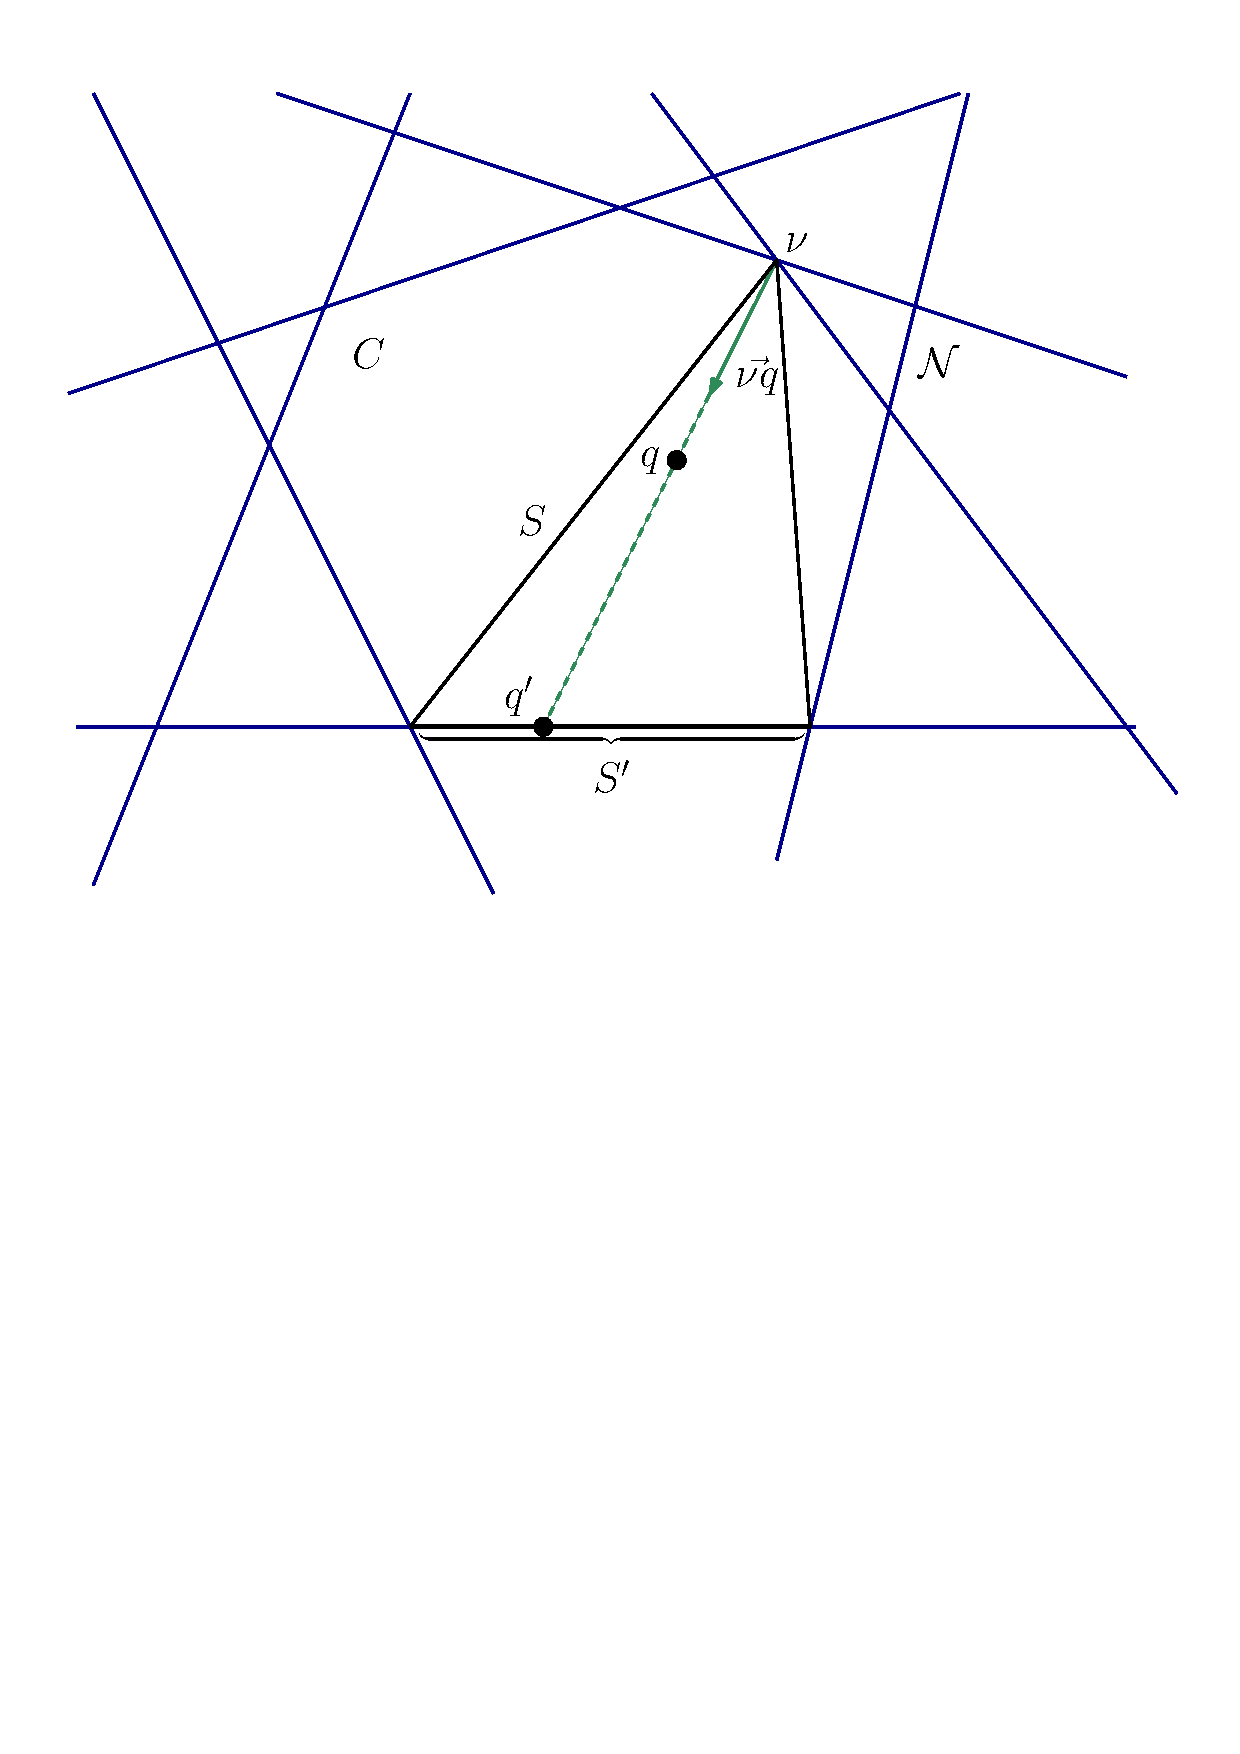
\includegraphics[trim=90 47 50 13,clip=true,height=0.25\textheight]{figures/simplex}
\caption{%
Illustration of a step of Algorithm~\ref{algo:simplex}.
}
\label{fig:meiser:step}
\end{center}
\end{figure}

\subsubsection{Assembling the pieces}

Let us summarize the algorithm
\begin{algorithm}\label{algo:meiser}
\item[input] \(q \in {[-1,1]}^n\)
\item[1.] Pick \(O(n^2 \log n)\) hyperplanes of $\Hy$ at random and locate $q$
in this arrangement. Call $\cell$ the cell containing $q$.
\item[2.] Construct the simplex \(\simplex\) containing \(q\) and inscribed in
\(\cell\), using Algorithm~\ref{algo:simplex}.
\item[3.] For every hyperplane of $\Hy$ containing $\simplex$, output a solution.
\item[4.] Recurse on hyperplanes of $\Hy$ intersecting the interior of $\simplex$.
\end{algorithm}

The query complexity of step \step{1} is $O(n^2 \log n)$, and that of step
\step{2} is $O(n^3 \log n)$. Steps \step{3} and \step{4} do not involve any
query at all. The recursion depth is $O(\log \card{\Hy})$, with $|\Hy|=O(n^k)$,
hence the total query complexity of this algorithm is $O(n^3 \log^2 n)$. This
proves the first part of Theorem~\ref{thm:cube}.\\

We can also consider the overall complexity of the algorithm in the RAM model,
that is, taking into account the steps that do not require any query, but for
which we still have to process the set $\Hy$. Note that the complexity
bottleneck of the algorithm are steps \step{3}-\step{4}, where we need to prune
the list of hyperplanes according to their relative positions with respect to
$\simplex$. For this purpose, we simply maintain explicitly the list of all
hyperplanes, starting with the initial set corresponding to all $k$-tuples.
Then the pruning step can be performed by looking at the position of each
vertex of $\simplex$ relative to each hyperplane of $\Hy$.
Because in our case hyperplanes have only $k$ nonzero coefficients, this uses a
number of integer arithmetic operations on $\tilde{O}(n)$ bits integers that is
proportional to the number of vertices times the number of hyperplanes.
(For the justification of the bound on the number of bits needed to represent
vertices of the arrangement see Appendix~\ref{app:bound}.)
Since we recurse on a fraction of the set, the overall complexity is
$\tilde{O}(n^2\card{\Hy}) = \tilde{O}(n^{k+2})$. The next section is devoted
to improving this running time.


